% IPR Technical Documentation -- compile with latexmk or pdflatex/bibtex.
\documentclass[12pt,a4paper,oneside]{report}

\usepackage[T1]{fontenc}
\usepackage[utf8]{inputenc}
\usepackage[english]{babel}
\usepackage{lmodern}
\usepackage{microtype}
\usepackage{setspace}
\onehalfspacing
\setlength{\parindent}{0pt}
\setlength{\parskip}{0.5\baselineskip}
\setlength{\emergencystretch}{2em}
\usepackage[a4paper,margin=2.35cm]{geometry}
\usepackage{graphicx}
\usepackage{booktabs}
\usepackage{longtable}
\usepackage{array}
\usepackage{amsmath,amssymb,mathtools}
\usepackage{xcolor}
\usepackage{hyperref}
\usepackage{tikz}
\usetikzlibrary{arrows.meta,positioning,shapes.geometric,fit,calc,backgrounds}

\hypersetup{
  pageanchor=false,
  colorlinks=true,
  linkcolor=blue!55!black,
  citecolor=blue!55!black,
  urlcolor=blue!55!black,
  pdftitle={Technical Documentation -- IPR},
  pdfauthor={IPR Project}
}

\definecolor{iprblue}{HTML}{1F4E79}
\definecolor{iprgreen}{HTML}{2D6A4F}
\definecolor{iprgray}{HTML}{5B6573}
\tikzset{
  component/.style={draw=iprblue, rounded corners=2pt, fill=blue!4, align=center, minimum height=8mm, text width=33mm},
  service/.style={draw=iprgreen!80!black, rounded corners=2pt, fill=green!5, align=center, minimum height=8mm, text width=34mm},
  storage/.style={draw=iprgray, cylinder, shape border rotate=90, aspect=0.28, fill=gray!8, align=center, minimum height=8mm, text width=29mm},
  actor/.style={draw=iprblue, rounded corners=9pt, fill=blue!6, align=center, minimum width=27mm, minimum height=8mm},
  flow/.style={-{Stealth[length=2.2mm]}, thick, iprgray},
  message/.style={-{Stealth[length=1.8mm]}, thin, iprblue}
}

\newcommand{\IPR}{\textsc{ipr}}

\begin{document}

\begin{titlepage}
\centering
\vspace*{2.7cm}
{\Huge\bfseries Technical Documentation\par}
\vspace{0.35cm}
{\LARGE \IPR{} -- Image Processing and Rendering\par}
\vspace{1.2cm}
{\large Architecture, RAW Development Pipeline, Interface, and Persistence\par}
\vfill
\begin{tabular}{rl}
Version & 0.3 -- RAW Restoration as of October 8, 2026\\
Status & Living Document -- Versioned LaTeX Sources\\
Scope & Windows 10/11 Desktop Application, Qt 6, C++ and QML
\end{tabular}
\vfill
{\small Chapters not yet started are present as intentionally empty placeholders.}
\end{titlepage}

\pagenumbering{roman}
\hypersetup{pageanchor=true}
\tableofcontents
\clearpage
\pagenumbering{arabic}

\chapter{Project Overview}
\label{chap:projet}

\section{Objective}

\IPR{} is a non-destructive photographic development software. It opens a folder or an image, decodes RAW files and supported image formats, displays a working image, and allows building an exportable render using photographic adjustments. The application targets local execution on Windows~10 and Windows~11, with a Qt Quick/QML interface and a C++ engine.

The guiding principle is to preserve the source file: the pixels of the original file are never overwritten. Settings, curves, and annotation metadata are stored in a companion \texttt{.ipr} file. Rendering is recalculated from the decoded image and current parameters.

\section{Current Functional Scope}

\begin{longtable}{p{0.30\linewidth}p{0.62\linewidth}}
\toprule
Function & Status and Responsibility \\
\midrule
Opening & Folder or image selection; opening an image switches to its parent folder. \\
Navigation & Horizontal thumbnail ribbon, deferred loading, and preloading of neighboring images. \\
Development & Exposure, tone, white balance, global color, local detail, haze, grain, curves, color mixer, and color grading. \\
User Metadata & Note, color label, and flag associated with the image. \\
Persistence & Atomic \texttt{.ipr} sidecar; automatic restoration when the source file is unchanged. \\
Batch & Multi-selection and application of current image settings to selected images. \\
Profiles & Local search for DCP/LCP profiles indexed in \texttt{profiles/index.json}. \\
Export & Rendered image exportable and automated export tests. \\
\bottomrule
\end{longtable}

\section{Architecture Constraints and Principles}

\begin{itemize}
  \item \textbf{Responsiveness:} Expensive decoding must not block the interface; loading is asynchronous and intermediate renders are deferred.
  \item \textbf{Bounded Memory:} The decoded image cache follows an LRU policy to limit memory consumption during long navigation.
  \item \textbf{Fidelity:} Photometric operations are performed in a linear floating-point working image when the pipeline allows.
  \item \textbf{Portability:} The distributed target is Windows, while the project can be built and tested in a WSL development environment.
  \item \textbf{Traceability:} Validation reports and measurements are organized in \texttt{docs/validation}, while dated logs reside in \texttt{docs/reports}. The documentary entry point is \texttt{docs/INDEX.md}.
\end{itemize}

\section{Scope Limitations}

Cropping, geometry, retouching masks, and AI-assisted functions already have reserved chapters in this document but are not yet implemented in the scope described here. Their lack of content is intentional to avoid documenting an unvalidated design as an existing feature.

\chapter{Architecture and Data Flow}
\label{chap:architecture}

\section{Overview}

The QML interface constitutes the presentation layer. It delegates opening, settings, navigation, and export to \texttt{ImageEditor}, a C++ object exposed to QML. The engine orchestrates the cache, decoding, profiles, and color pipeline. Results are made available to QML via an image provider and a thumbnail provider.

\begin{figure}[htbp]
\centering
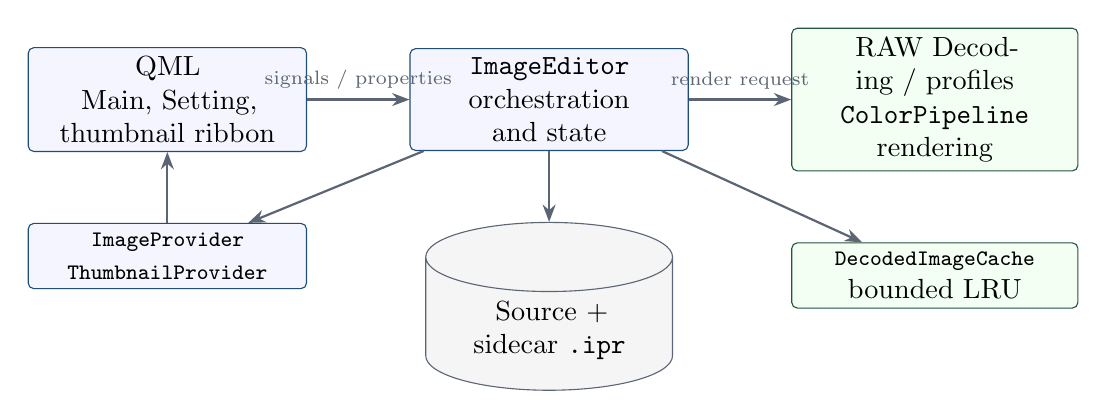
\begin{tikzpicture}[node distance=9mm and 13mm]
  \node[component] (qml) {QML\\Main, Setting, thumbnail ribbon};
  \node[component, right=of qml] (editor) {\texttt{ImageEditor}\\orchestration and state};
  \node[service, right=of editor] (pipeline) {RAW Decoding / profiles\\\texttt{ColorPipeline}\\rendering};
  \node[service, below=of pipeline] (cache) {{\footnotesize\texttt{DecodedImageCache}}\\bounded LRU};
  \node[storage, below=of editor] (sidecar) {Source +\\sidecar \texttt{.ipr}};
  \node[component, below=of qml] (providers) {{\footnotesize\texttt{ImageProvider}}\\{ \footnotesize\texttt{ThumbnailProvider}}};
  \draw[flow] (qml) -- node[above, font=\scriptsize]{signals / properties} (editor);
  \draw[flow] (editor) -- node[above, font=\scriptsize]{render request} (pipeline);
  \draw[flow] (editor) -- (sidecar);
  \draw[flow] (editor) -- (cache);
  \draw[flow] (editor) -- (providers);
  \draw[flow] (providers) -- (qml);
\end{tikzpicture}
\caption{Logical architecture of \IPR{}.}
\end{figure}

\section{Global Presentation Preferences}

The C++ service \texttt{UiPreferences}, exposed to QML separately from \texttt{ImageEditor}, preserves the interface state in the user file \texttt{ipr-ui.ini}. The path is resolved by \texttt{QStandardPaths}, via \texttt{AppConfigLocation}, not by the photos folder. Schema 2 is validated on loading; the old magenta selection (index 6) is migrated to 7 from schema 1. A file with a newer version remains unchanged and read-only. Writes are grouped for 400~ms and synchronized on close by \texttt{QSettings::IniFormat}, with atomic synchronization required~\cite{qtQSettings,qtQStandardPaths}. Normal geometry is preserved independently of maximized or full-screen state; the window is repositioned on an available screen at restart. The full contract is described in \texttt{docs/architecture/ui-preferences.md}. Since the portable build of October 8, the presence of \texttt{config/ipr-ui.ini} next to the executable takes priority over this user path. The local RAW manifest can reside in \texttt{config/raw-normalization.json}; these two files have distinct roles.

\section{Working Image and Ordering}

The working image is a floating-point RGBA representation, \texttt{WorkingImage}. It avoids premature rounding errors and allows values greater than~1 before output encoding. The engine applies corrections in an explicit order:

\begin{enumerate}
  \item RAW decoding, possible controlled normalization, LCP then DCP;
  \item grayscale levels, exposure, contrast;
  \item temperature/tint, shadows, blacks, highlights, and whites;
  \item vibrance/saturation, mixer, and color grading;
  \item noise reduction, texture, clarity, and haze correction;
  \item luminance/RGB curves, blur, sharpening, and grain;
  \item gamut mapping and output encoding.
\end{enumerate}

Camera WB is applied during decoding; the temperature/tint sliders are an additional adjustment of the working RGB. They must not be confused with the initial WB. The above order describes the path with DCP; without DCP, the LCP acts on the linear sRGB provided by LibRaw. Renders are grouped by timeout during cursor manipulation.

\section{Zoom and Before/After Comparison}

The \texttt{ImageViewport.qml} component displays the working proxy with zoom and displacement common to both renders. The Before/After button, also accessible via Ctrl+Shift+C, separates the origin on the left from the current render on the right. A movable border defines two complementary clips, without double alpha composition. 100\% zoom focuses on proxy pixels (largest side limited to 2048 pixels), not full-resolution RAW.

The reference is the already decoded, profiled, and developed source by IPR, encoded in 8-bit sRGB without editor or sidecar settings. It is not the JPEG embedded in the RAW. Its conversion is calculated in the background at the first accepted render, then reused during adjustments. \texttt{ImageProvider} publishes the pair under lock before QML notification; \texttt{originalImageSource} preserves a stable URL, unlike \texttt{imageSource}, revised with each render. On source change, both references are cleared. An automatic white balance re-decoding also renews this origin.

The additional CPU storage of the provider is at most a 16~Mpx preview, excluding Qt Quick resources; no additional RAW is decoded to enable comparison. Zoom, mode, and separation are not persisted in INI or sidecar. Histogram and export remain those of the current render. The detailed contract is in \texttt{docs/specifications/zoom-image.md}.

\section{Cache and Memory Lifetime}

\texttt{DecodedImageCache} preserves recent decoded images according to a \emph{Least Recently Used} (LRU) policy. Accessing an image makes it the most recent; when an insertion exceeds capacity, the least recently used entry is released. This mechanism separates decoding cost from rendering cost and prevents large folder exploration from indefinitely monopolizing memory.

Thumbnails follow a separate policy: the view loads visible elements and a preloading neighborhood, currently estimated at four images before and after the visible area. Elements too far away are evicted. This number remains a performance parameter to be measured on target corpora.

\section{Camera and Lens Profiles}

DCP (camera color rendering) and LCP (lens correction) profiles are searched in a local indexed library. This strategy accelerates profile resolution and avoids repeated exploration of the installation tree. Profile files must come from a source whose license explicitly allows their redistribution; the local index does not constitute authorization to copy profiles from a third-party product.

\section{Controlled RAW Development}

\texttt{RawDevelopmentModule.qml} allows choosing a compatible DCP, modifying automatic WB, and checking experimental normalization. \texttt{RawNormalization::resolve()} verifies a bounded manifest, RAW/DCP SHA-256, ISO, blacks, camera body, and LibRaw version. The base exposure gain and audited white are applied only after validation; a refusal preserves the uncalibrated path. Cache keys distinguish profile and manifest.

Camera Neutral is visually accepted on the local corpus, without Lightroom parity or certified physical fidelity. Adobe Standard remains to be processed. The current calibration concerns five exact files; it does not constitute a general rule for the R6 Mark III. The v5 sidecar preserves the profile, manifest, their SHA-256, activation, and engine/LibRaw version. These choices and automatic WB are restored before decoding. The LCP remains automatic and is not yet fixed in the recipe.

Changing DCP is a retouch: an active pre-DCP camera buffer (384 MB maximum, outside LRU) allows applying the new profile without re-executing LibRaw. Preview, zoom, and settings remain available. RAW WB, calibration, or lack of buffer still require decoding. An error preserves the previous base. Resets of retouches and profile/calibration are separate.

\chapter{User Diagram and Workflow}
\label{chap:utilisateur}

\section{Use Cases}

\begin{figure}[htbp]
\centering
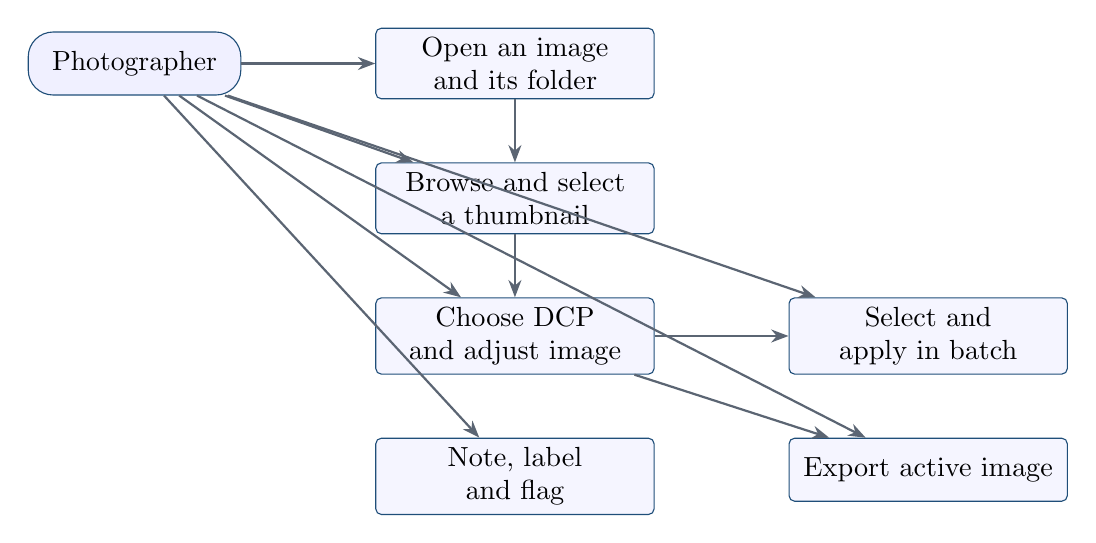
\begin{tikzpicture}[node distance=8mm and 17mm]
  \node[actor] (user) {Photographer};
  \node[component, right=of user] (open) {Open an image\\and its folder};
  \node[component, below=of open] (browse) {Browse and select\\a thumbnail};
  \node[component, below=of browse] (adjust) {Choose DCP\\and adjust image};
  \node[component, below=of adjust] (meta) {Note, label\\and flag};
  \node[component, right=of adjust] (batch) {Select and\\apply in batch};
  \node[component, below=of batch] (export) {Export active image};
  \draw[flow] (user) -- (open);
  \draw[flow] (user) -- (browse);
  \draw[flow] (user) -- (adjust);
  \draw[flow] (user) -- (meta);
  \draw[flow] (user) -- (batch);
  \draw[flow] (user) -- (export);
  \draw[flow] (open) -- (browse);
  \draw[flow] (browse) -- (adjust);
  \draw[flow] (adjust) -- (batch);
  \draw[flow] (adjust) -- (export);
\end{tikzpicture}
\caption{Existing actions. Batch application of settings is not batch export.}
\end{figure}

\section{Nominal Workflow}

\begin{enumerate}
  \item The user selects \emph{Open}. They can directly select an image; \IPR{} then opens the folder containing it and activates the chosen image.
  \item The bottom ribbon displays thumbnails. A selected image becomes the working image; the information panel exposes its properties.
  \item On a RAW, the RAW Development / Profile module exposes compatible DCPs. The status distinguishes requested normalization from effectively applied normalization.
  \item Adjustment commands modify the state of \texttt{ImageEditor}. The numeric field and slider represent the same value and must remain synchronized.
  \item After interaction stops, the render is updated, then settings are written to the sidecar. Changing an image restores its own settings or neutral values in the absence of a sidecar.
  \item The user can check multiple thumbnails and apply the settings of the active image to the selection. Each image then receives its own sidecar.
  \item Export processes the active image at full resolution. The export queue for an entire selection remains to be implemented.
\end{enumerate}

\section{Ergonomics Requirements}

The settings panel is fixed to the right edge and must not obscure the image. Scroll bars and sliders are intentionally discreet, but numeric fields remain editable to allow precise input. Controls exclusively reset their target setting.

\chapter{Class Diagrams}
\label{chap:classes}

\section{Rendering and Image Access Classes}

\begin{figure}[htbp]
\centering
\resizebox{\textwidth}{!}{%
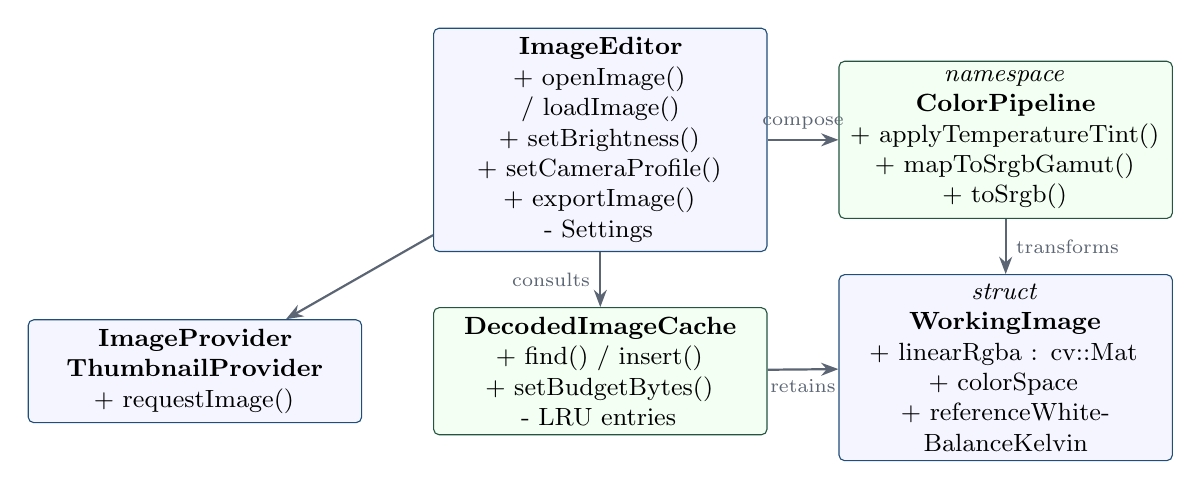
\begin{tikzpicture}[node distance=7mm and 9mm, every node/.style={font=\small}]
  \node[component, text width=40mm] (editor) {\textbf{ImageEditor}\\+ openImage() / loadImage()\\+ setBrightness()\\+ setCameraProfile()\\+ exportImage()\\- Settings};
  \node[service, right=of editor, text width=40mm] (pipeline) {\textit{namespace}\\\textbf{ColorPipeline}\\+ applyTemperatureTint()\\+ mapToSrgbGamut()\\+ toSrgb()};
  \node[service, below=of editor, text width=40mm] (cache) {\textbf{DecodedImageCache}\\+ find() / insert()\\+ setBudgetBytes()\\- LRU entries};
  \node[component, below=of pipeline, text width=40mm] (working) {\textit{struct}\\\textbf{WorkingImage}\\+ linearRgba : cv::Mat\\+ colorSpace\\+ referenceWhiteBalanceKelvin};
  \node[component, left=of cache, text width=40mm] (provider) {\textbf{ImageProvider}\\\textbf{ThumbnailProvider}\\+ requestImage()};
  \draw[flow] (editor) -- node[above, font=\scriptsize]{compose} (pipeline);
  \draw[flow] (pipeline) -- node[right, font=\scriptsize]{transforms} (working);
  \draw[flow] (editor) -- node[left, font=\scriptsize]{consults} (cache);
  \draw[flow] (cache) -- node[below, font=\scriptsize]{retains} (working);
  \draw[flow] (editor) -- (provider);
\end{tikzpicture}
}
\caption{Rendering core and Qt Quick providers.}
\end{figure}

\section{Settings and Persistence Classes}

\begin{figure}[htbp]
\centering
\resizebox{\textwidth}{!}{%
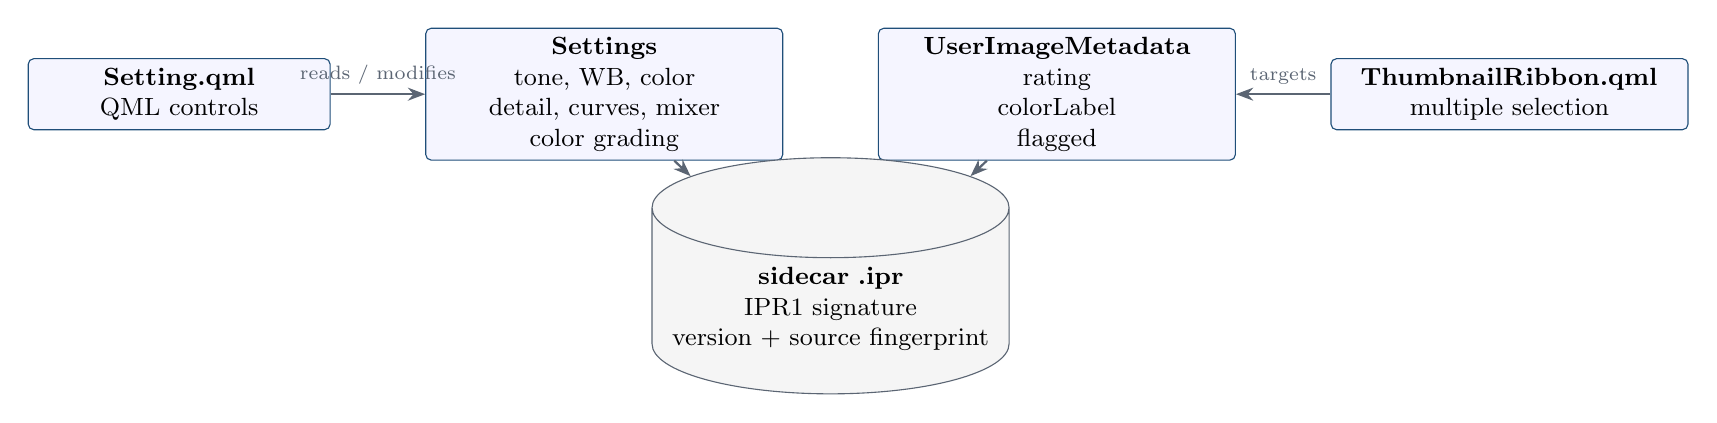
\begin{tikzpicture}[node distance=8mm and 12mm, every node/.style={font=\small}]
  \node[component, text width=43mm] (settings) {\textbf{Settings}\\tone, WB, color\\detail, curves, mixer\\color grading};
  \node[component, right=of settings, text width=43mm] (metadata) {\textbf{UserImageMetadata}\\rating\\colorLabel\\flagged};
  \coordinate (persistenceCenter) at ($(settings)!0.5!(metadata)$);
  \node[storage, below=of persistenceCenter, text width=43mm] (ipr) {\textbf{sidecar .ipr}\\IPR1 signature\\version + source fingerprint};
  \node[component, left=of settings, text width=36mm] (qml) {\textbf{Setting.qml}\\QML controls};
  \node[component, right=of metadata, text width=43mm] (ribbon) {\textbf{ThumbnailRibbon.qml}\\multiple selection};
  \draw[flow] (qml) -- node[above, font=\scriptsize]{reads / modifies} (settings);
  \draw[flow] (settings) -- (ipr);
  \draw[flow] (metadata) -- (ipr);
  \draw[flow] (ribbon) -- node[above, font=\scriptsize]{targets} (metadata);
\end{tikzpicture}
}
\caption{Editable state, annotations, and non-destructive persistence.}
\end{figure}

\section{Responsibilities}

The main provider \texttt{ImageProvider} exposes the current render and the neutral reference via \texttt{requestImage()}, \texttt{image()}, and \texttt{originalImage()}. \texttt{setImages()} publishes the pair under lock. The \texttt{originalImageSource} property of \texttt{ImageEditor} signals its availability to QML. The \texttt{ImageViewport.qml} component carries only the navigation and comparison state; it does not modify \texttt{Settings}.

\texttt{ImageEditor} owns the active state and orchestrates rendering in \texttt{renderWorkingImage()}. The functions of the \texttt{ColorPipeline} namespace ensure conversions, adaptation, and gamut; \texttt{ColorMixer} and \texttt{DetailProcessing} carry their specialized processing. \texttt{DecodedImageCache} retains source, proxy, and metadata, without QML state. The indicated methods correspond to current C++ headers; namespaces are not presented as instantiable classes.

\section{Profiles, Normalization, and Preferences}

\begin{figure}[htbp]
\centering
\resizebox{\textwidth}{!}{%
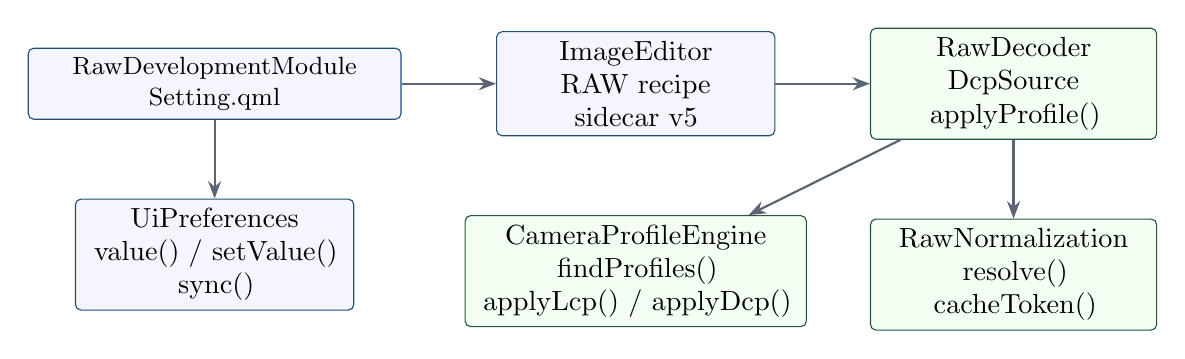
\begin{tikzpicture}[node distance=10mm and 12mm]
  \node[component,text width=45mm,font=\small] (ui) {RawDevelopmentModule\\Setting.qml};
  \node[component, right=of ui] (editor) {ImageEditor\\RAW recipe\\sidecar v5};
  \node[service, right=of editor] (raw) {RawDecoder\\DcpSource\\applyProfile()};
  \node[service, below=of raw] (normal) {RawNormalization\\resolve()\\cacheToken()};
  \node[service, below=of editor,text width=41mm] (profiles) {CameraProfileEngine\\findProfiles()\\applyLcp() / applyDcp()};
  \node[component, below=of ui] (prefs) {UiPreferences\\value() / setValue()\\sync()};
  \draw[flow] (ui) -- (editor);
  \draw[flow] (editor) -- (raw);
  \draw[flow] (raw) -- (normal);
  \draw[flow] (raw) -- (profiles);
  \draw[flow] (ui) -- (prefs);
\end{tikzpicture}}
\caption{RAW contracts and presentation. The INI preserves UI; the v5 sidecar preserves DCP and calibration choices per image.}
\end{figure}

\chapter{Sequence Diagrams}
\label{chap:sequences}

\section{Image Opening}

\begin{figure}[htbp]
\centering
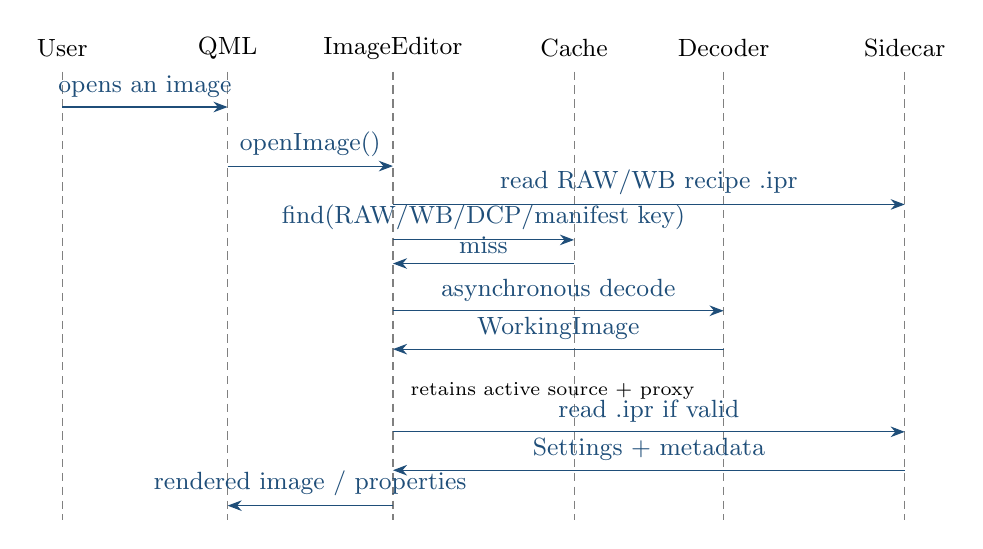
\begin{tikzpicture}[x=1cm,y=0.75cm,font=\small]
  \foreach \x/\name in {0/User,2.1/QML,4.2/ImageEditor,6.5/Cache,8.4/Decoder,10.7/Sidecar} {
    \node[align=center] at (\x,0) {\name};
    \draw[densely dashed,gray] (\x,-0.4) -- (\x,-8.0);
  }
  \draw[message] (0,-1) -- node[above,sloped]{opens an image} (2.1,-1);
  \draw[message] (2.1,-2) -- node[above,sloped]{openImage()} (4.2,-2);
  \draw[message] (4.2,-2.65) -- node[above,sloped]{read RAW/WB recipe .ipr} (10.7,-2.65);
  \draw[message] (4.2,-3.25) -- node[above,sloped]{find(RAW/WB/DCP/manifest key)} (6.5,-3.25);
  \draw[message] (6.5,-3.65) -- node[above,sloped]{miss} (4.2,-3.65);
  \draw[message] (4.2,-4.45) -- node[above,sloped]{asynchronous decode} (8.4,-4.45);
  \draw[message] (8.4,-5.1) -- node[above,sloped]{WorkingImage} (4.2,-5.1);
  \node[align=left,anchor=west,font=\scriptsize] at (4.3,-5.8) {retains active source + proxy};
  \draw[message] (4.2,-6.5) -- node[above,sloped]{read .ipr if valid} (10.7,-6.5);
  \draw[message] (10.7,-7.15) -- node[above,sloped]{Settings + metadata} (4.2,-7.15);
  \draw[message] (4.2,-7.75) -- node[above,sloped]{rendered image / properties} (2.1,-7.75);
\end{tikzpicture}
\caption{Cache miss path. The old inactive RAW is inserted into the LRU at transition, not systematically the new active RAW.}
\end{figure}

\section{Adjustment and Batch Application}

\begin{figure}[htbp]
\centering
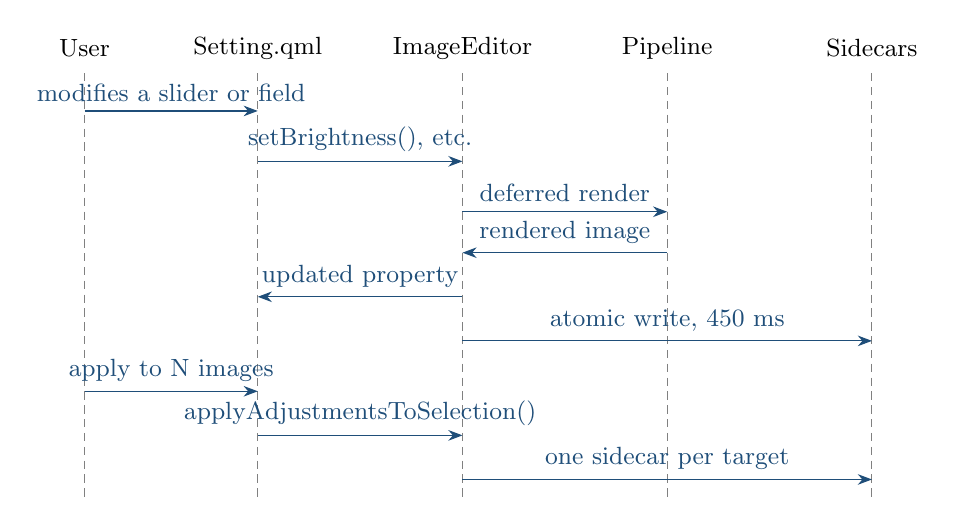
\begin{tikzpicture}[x=1cm,y=0.8cm,font=\small]
  \foreach \x/\name in {0/User,2.2/Setting.qml,4.8/ImageEditor,7.4/Pipeline,10.0/Sidecars} {
    \node[align=center] at (\x,0) {\name};
    \draw[densely dashed,gray] (\x,-0.4) -- (\x,-7.2);
  }
  \draw[message] (0,-1) -- node[above,sloped]{modifies a slider or field} (2.2,-1);
  \draw[message] (2.2,-1.8) -- node[above,sloped]{setBrightness(), etc.} (4.8,-1.8);
  \draw[message] (4.8,-2.6) -- node[above,sloped]{deferred render} (7.4,-2.6);
  \draw[message] (7.4,-3.25) -- node[above,sloped]{rendered image} (4.8,-3.25);
  \draw[message] (4.8,-3.95) -- node[above,sloped]{updated property} (2.2,-3.95);
  \draw[message] (4.8,-4.65) -- node[above,sloped]{atomic write, 450 ms} (10.0,-4.65);
  \draw[message] (0,-5.45) -- node[above,sloped]{apply to N images} (2.2,-5.45);
  \draw[message] (2.2,-6.15) -- node[above,sloped]{applyAdjustmentsToSelection()} (4.8,-6.15);
  \draw[message] (4.8,-6.85) -- node[above,sloped]{one sidecar per target} (10.0,-6.85);
\end{tikzpicture}
\caption{Non-destructive adjustment cycle and voluntary propagation to a selection.}
\end{figure}

\section{Profile Change and Normalization}

\begin{figure}[htbp]
\centering
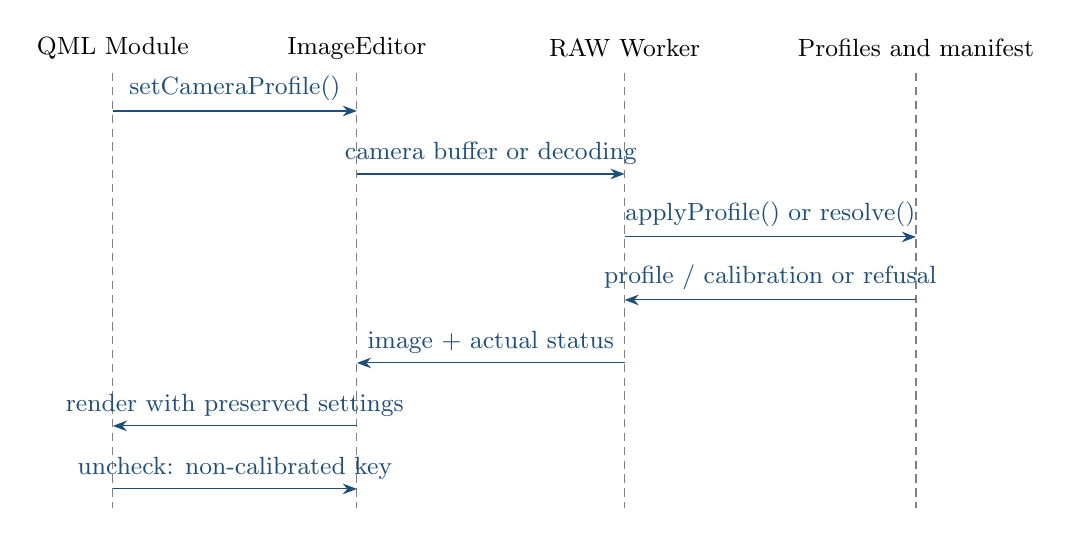
\begin{tikzpicture}[x=1cm,y=0.8cm,font=\small]
  \foreach \x/\name in {0/QML Module,3.1/ImageEditor,6.5/RAW Worker,10.2/Profiles and manifest} {
    \node[align=center] at (\x,0) {\name};
    \draw[densely dashed,gray] (\x,-0.4) -- (\x,-7.3);
  }
  \draw[message] (0,-1) -- node[above]{setCameraProfile()} (3.1,-1);
  \draw[message] (3.1,-2) -- node[above]{camera buffer or decoding} (6.5,-2);
  \draw[message] (6.5,-3) -- node[above]{applyProfile() or resolve()} (10.2,-3);
  \draw[message] (10.2,-4) -- node[above]{profile / calibration or refusal} (6.5,-4);
  \draw[message] (6.5,-5) -- node[above]{image + actual status} (3.1,-5);
  \draw[message] (3.1,-6) -- node[above]{render with preserved settings} (0,-6);
  \draw[message] (0,-7) -- node[above]{uncheck: non-calibrated key} (3.1,-7);
\end{tikzpicture}
\caption{The pre-DCP buffer avoids LibRaw when WB/calibration allows. The visible render remains preserved; the v5 recipe is saved after success. The checkbox alone does not guarantee calibration.}
\end{figure}

\chapter{Already Integrated Adjustments}
\label{chap:reglages-existants}

\section{Calculation Convention}

The pipeline manipulates a pixel $\mathbf{p}=(r,g,b)^T$ in floating-point values. Photometric calculations must be performed on linear components; sRGB encoding or export format is applied at the end. The relative luminance used for normalizations is:
\begin{equation}
  Y = 0.2126r + 0.7152g + 0.0722b.
\end{equation}

The formula is that of Rec.~709/sRGB. Maintaining floating-point precision before encoding reduces detail loss in highlights and avoids unnecessary intermediate saturations.

\section{Global Tonality}

\subsection{Exposure, Contrast, and Tone}

Exposure in IL (EV) values is a multiplicative gain:
\begin{equation}
  \mathbf{p}' = 2^{E}\mathbf{p},
\end{equation}
where $E$ is the exposure setting. A change of $+1$~EV thus doubles the energy of linear components.

Contrast and \emph{highlights}, \emph{shadows}, \emph{whites}, and \emph{blacks} settings are driven by luminance weighting functions. Generically, a local tone correction takes the form:
\begin{equation}
  Y' = Y + a\,w(Y),
\end{equation}
where $a$ is the requested intensity and $w$ a soft window focused on the targeted range. Components are then rescaled with chromaticity preservation. This approach prevents a shadow adjustment from affecting highlights as much.

Validation tests performed on the reference corpus have validated the EV slider as well as shadow, black, white, and highlight adjustments. The matrix, analyses, and measurement files are organized in \texttt{docs/validation}; historical evidence remains consultable during documentary migration.

\subsection{Curves}

Available curves are a luminance curve and Red, Green, and Blue curves. Between control points $(x_i,y_i)$, the implementation relies on Lagrange polynomial interpolation:
\begin{equation}
  P(x)=\sum_{i=0}^{n} y_i\prod_{j\ne i}\frac{x-x_j}{x_i-x_j}.
\end{equation}

Channel curves allow creative tinting, while the luminance curve adjusts tonal contrast. HDR values are extended linearly beyond the control interval to avoid introducing abrupt cuts.

\section{White Balance and Tint}

Temperature is calculated from the correlated Planckian locus according to Krystek's algorithm~\cite{krystek1985}. Chromaticity gains are applied using Bradford chromatic adaptation~\cite{lam1985}, formulated matricially:
\begin{equation}
 \mathbf{RGB}' = M_{XYZ\rightarrow RGB}\,B^{-1}\,D\,B\,M_{RGB\rightarrow XYZ}\,\mathbf{RGB},
\end{equation}
where $B$ is the Bradford matrix and $D$ a diagonal matrix of ratios between reference white and target white in LMS space.

Tint compensates the green-magenta axis. Colored gains are normalized to preserve luminance as much as possible:
\begin{equation}
  n=0.2126r_g+0.7152g_g+0.0722b_g, \qquad \mathbf{p}'=\frac{\mathbf{g}\odot\mathbf{p}}{n}.
\end{equation}
Temperature validation is recorded in the protocol and analyses of October 2, 2026.

\section{Global Color, Color Mixer, and Color Grading}

\subsection{Vibrance and Saturation}

Saturation adjusts chromatic amplitude uniformly. Vibrance protects already saturated colors more. If $c=(\max(r,g,b)-\min(r,g,b))/\max(r,g,b)$ is the relative chroma, an approximation of the vibrance gain is:
\begin{equation}
  g_v = 1+\frac{V}{100}(1-c).
\end{equation}
Thus, low-saturation colors receive most of the effect. Vibrance and saturation controls have undergone basic verifications preceding mixer and grading work.

\subsection{Color Mixer}

The C++ \texttt{ColorMixer} module operates in an HSV representation of linear RGB on eight bands: red, orange, yellow, green, cyan, blue, violet, and magenta. The centers, in degrees, are:
\[0,\;30,\;60,\;120,\;180,\;240,\;270,\;300.\]
For an original hue $h$, the influence of a band centered at $h_i$ is triangular:
\begin{equation}
  w_i(h)=\max\left(0,1-\frac{|\delta_i(h)|}{a_i(h)}\right),
\end{equation}
where $\delta_i(h)$ is the signed circular distance in $[-180^\circ,180^\circ]$ and $a_i(h)$ the distance from the center to the neighboring center on the considered side. Weights are calculated on the source hue and multiplied by $q=t^2(3-2t)$, with $t=\operatorname{clamp}(S/0.05,0,1)$, to protect achromatics. Weighted commands are added before application, without multiplied gains at overlaps.
\begin{align}
 H'&=H+18^\circ\sum_i qw_iH_i/100,\\
 S'&=\operatorname{clamp}\left(S\left[1+\sum_i qw_iS_i/100\right],0,1\right),\\
 Y'&=Y\,2^{0.5\sum_i qw_iL_i/100}.
\end{align}
HSV reconversion is normalized to the source luminance before selective gain. The bounds $\pm100$ guarantee a gain between $1/\sqrt{2}$ and $\sqrt{2}$. The chroma threshold $0.05$ and the bound $0.5$ EV are initial empirical choices, not a validated Lightroom calibration. Grays are exactly unchanged, and negative channels are not clipped in this module. Output gamut mapping may modify $Y$. The mixer and grading remain independent of global saturation and vibrance; a zero mixer does not change the base render.

\subsection{Color Grading}

Three independent zones are available: shadows, midtones, and highlights. They receive a color defined by hue and saturation. A smooth function of $Y$ distributes the influence of each zone; chromatic correction is added with intensity proportional to saturation, then bounded at export time. This solution is intentionally lightweight and non-destructive; future visual validation must specify its limits at high saturation.

\section{Local Detail, Haze, and Grain}

\subsection{Texture and Clarity}

Texture and clarity rely on the detail component of a Gaussian blur decomposition:
\begin{equation}
  D_\sigma = Y-G_\sigma(Y), \qquad Y'=Y+aD_\sigma w(Y),
\end{equation}
where $G_\sigma$ is a Gaussian blur. Texture uses a short scale ($\sigma\approx1.2$), clarity a wider scale ($\sigma\approx8$). Protection weights limit enhancement in extremes and very low chromaticity areas. The blur primitive is consistent with that documented by OpenCV~\cite{opencvGaussian}.

\subsection{Haze Correction}

The simplified physical model by Koschmieder relates observation $I$, scene radiance $J$, atmospheric light $A$, and transmission $t$:
\begin{equation}
  I(x)=J(x)t(x)+A(1-t(x)).
\end{equation}
The estimation by \emph{dark channel prior} uses locally $\min_c I_c$ then reconstructs $J$ after estimation and bounding of $t$~\cite{he2009,he2011}. The implementation applies this logic as a gradual correction to avoid halos.

\subsection{CPU Noise Reduction and Sharpening}

\paragraph{Consolidation of October 5, 2026.}

Denoising precedes local effects and sharpening. It separates linear RGB into $Y=0.2126R+0.7152G+0.0722B$, $Co=R-B$, and $Cg=G-(R+B)/2$. Planes have a distinct noise estimate by the MAD of the Haar diagonal detail $(p_{00}-p_{01}-p_{10}+p_{11})/2$, normalized by $0.67448975$. Blocks exactly constant do not participate in this estimate; it remains a proxy after demosaicing, not a sensor model.

For $s=\operatorname{clamp}(v,0,100)/100$, residuals of two successive blurs ($\sigma=0.8$ then $1.8$ pixels) undergo a threshold $\lambda_f=\widehat\sigma ms$, with $m=2.55$ for Y and $3.15$ for Co/Cg; $\lambda_m=0.52\lambda_f$. A prefiltered guide and a normalized Sobel protect edges, including isolated luminescent chromatic boundaries. The result is blended with the original with weight $s$. Positive and negative changes are balanced to preserve the mean without adding an offset to blacks. These coefficients are empirical.

Reconstruction writes $RGB=Y+d$, where the luminance of $d$ is zero. If a channel becomes negative, reduce $d$ towards the gray of same Y, without HDR upper clamp. The color setting alone thus preserves linear luminance per pixel at floating precision. At noise 0/0, the path is exactly short-circuited. Preserving global mean does not prevent local drift; photographic validation is still required.

CPU sharpening is an unsharp mask on Y, with threshold relative to noise and local limitation of overshoots. Its historical estimator and calibration do not change in this correction. The native test \texttt{detailProcessingTests} covers synthetic regressions, not Lightroom parity or guaranteed fidelity of all textures.

\subsection{Grain}

Grain is deterministic pseudo-random noise, dependent on pixel position and setting intensity. Its determinism ensures that the same export produces the same result and avoids flickering between two successive renders.

\section{Persistence and Batch Adjustment}

Presentation state is not part of the photographic sidecar. The global file \texttt{ipr-ui.ini} stores open sections, channel/band/zone selections, main colors, visibility and dimensions of panels, as well as export format and quality. Restoration is protected against QML default value writes at startup; it does not modify development settings. Keys reserved for cropping, masks, AI, and GPU are inactive. The View menu provides access to panel visibility and INI path, which is customized with the application closed.

The sidecar uses an \texttt{IPR1} signature, version number, size, and modification date of the source file. It stores settings, curves, and user metadata via \texttt{QDataStream}~\cite{qtQDataStream}. Deferred writing of 450~ms goes through \texttt{QSaveFile}, which writes temporarily then validates the file atomically~\cite{qtQSaveFile}. A non-matching source fingerprint invalidates the sidecar rather than potentially applying settings to another file.

The current v4 format stores eight color mixer triplets. Versions v1/v2/v3 are read while preserving their colors: the old last triplet becomes magenta at index 7; violet, new index 6, starts at zero, as does orange for v1/v2. Values are preserved, but the new model changes the render of old non-zero settings. Old executables do not read v4. INI schema 2 similarly migrates the magenta interface selection 6 to 7, without modifying photo settings.

Batch application copies only development settings from the active image to checked images. Local annotations of the destination are preserved when they exist. This choice prevents a photographic correction from unintentionally overwriting an already established rating.

\chapter{Cropping and Geometric Effects}
\label{chap:recadrage-geometrie}
% Reserved chapter. No content until design and implementation have begun.

\chapter{Masks and Local Retouching}
\label{chap:masques-retouche}
% Reserved chapter. No content until design and implementation have begun.

\chapter{Artificial Intelligence Integration}
\label{chap:ia}
% Reserved chapter. No content until design and implementation have begun.

\chapter{Quality, Validation, and Evolutions}
\label{chap:qualite}

\section{Validation Status}

Fundamental adjustments have been compared to reference exports on an sRGB TIFF corpus: exposure, blacks, shadows, whites, highlights, contrast, and temperature. Measurements notably use per-pixel differences (MAE) and overlay inspections when dimensions and encoding allow. This method distinguishes a spatial offset from a rendering difference.

The eight-band mixer has campaigns at extremes and intermediate values. Noise v2 has measured progressivity on twelve scenes; this does not guarantee the preservation of all details. Color grading, curves, sharpening, grain/blur, and their interactions require a photographic recipe. V4 sidecars and application of settings to a selection are implemented; their manual completion remains open. Batch export is not implemented. DNG rendering is not certified as Lightroom-compatible.

As of October 8, Camera Neutral is visually accepted by the user. Normalization remains experimental, limited to five exact files and disabled by default. The complete WSL suite passes 17 out of 18 tests: the JPEG 9933 probe still fails (RGB MAE 25.1519 for a threshold of 25), outside calibrated mode. The five targeted Windows suites of the latest portable adaptation and the 76 Python analysis tests plus 12 selection tests succeed. These numbers are a dated snapshot, not a guarantee of future execution.

\section{Elements to Complete Before Distribution}

\begin{itemize}
  \item Establish reproducible test sets for each setting and record metrics in a structured format.
  \item Measure opening time on representative RAW files, peak memory, and actual efficiency of LRU cache and thumbnail preloading.
  \item Formalize DCP/LCP profile compatibility: origin, license, version, and redistribution rights for each file.
  \item Complete the v4 sidecar schema recipe and its migrations; define backup/conflicts and persistence of DCP/normalization choices.
  \item Add a non-regression test for profile rendering, batch rendering, and metadata.
  \item Document the final export format (depth, embedded ICC profile, EXIF/XMP metadata) and its usage conditions.
\end{itemize}

\section{Applied Documentary Governance}

Experimental reports are distributed between \texttt{docs/validation} (protocol, analysis, and measurements) and \texttt{docs/reports} (session log). This tree is the compilable normative documentation. Any completed feature must update its chapter, concerned diagrams, bibliographic references, validation matrix, and test scenario. Cross-cutting architectural decisions must be added to a short ADR (\emph{Architecture Decision Record}) to avoid depending exclusively on session reports.

\section{Exported Measurements and Reproducible Graphics}

\texttt{scripts/export\_documentation\_metrics.py} generates CSV by family and SVG graphics from immutable evidence. Each value preserves its source file, SHA-256 fingerprint, and JSON or textual location. The \texttt{docs/validation/metrics} directory is a derived view, not a new source of truth. Literal numbers extracted from a log do not become homogeneous metrics without interpretation of their context.

CPU times and rendering indicators are separate: the time curve represents only the historical Windows benchmark before/after parallelization. Tone responses by revision, noise reduction progressivity, and DCP deviations from Lightroom are not speed measurements. No current rendering, thumbnail, or export time is invented; campaigns remain necessary.

\chapter{Glossary}
\label{chap:glossaire}

\begin{longtable}{p{0.24\linewidth}p{0.68\linewidth}}
\toprule
Term & Definition \\
\midrule
\endhead
\textbf{DCP} & \emph{DNG Camera Profile}. Profile that notably describes a color transformation related to a camera body. \\
\textbf{LCP} & \emph{Lens Correction Profile}. Optical lens correction profile (distortion, vignetting, aberration according to the profile). \\
\textbf{EV / IL} & Exposure Value. An increment of +1 corresponds to a doubling of light energy in the linear model. \\
\textbf{HDR} & \emph{High Dynamic Range}. Working values beyond the usual display range, preserved before final encoding. \\
\textbf{ICC} & Standardized profile describing the color reproduction of a device or color space~\cite{icc2022}. \\
\textbf{LRU} & \emph{Least Recently Used}. Eviction policy that removes the element whose last access is the oldest. \\
\textbf{LMS} & Approximate response space of Long, Medium, and Short cones, used here for chromatic adaptation. \\
\textbf{MAE} & \emph{Mean Absolute Error}, average of absolute deviations between two images compared pixel by pixel. \\
\textbf{MAD} & \emph{Median Absolute Deviation}, median of absolute deviations from the median; robust estimator used for Haar coefficient noise. Do not confuse with MAE. \\
\textbf{CIEDE2000} & Color difference formula used here for Lab D65 comparisons. A low deviation from Lightroom does not prove physical fidelity. \\
\textbf{RAW Manifest} & JSON file of audited calibrations linked to RAW/DCP fingerprints and decoding context; distinct from the photographic sidecar. \\
\textbf{Derived CSV} & Regenerable tabular view of evidence; preserves source, location, and provenance, without replacing the original measurement. \\
\textbf{RAW} & Data from the sensor, before final photographic rendering. \\
\textbf{Sidecar} & Companion file carrying settings without modifying the source image file. \\
\textbf{sRGB} & Standard color space notably intended for screens and the web, defined by IEC~61966-2-1~\cite{srgb}. \\
\textbf{TIFF} & Image container format that can preserve different depths, compressions, and color profiles. \\
\bottomrule
\end{longtable}


\clearpage
\addcontentsline{toc}{chapter}{Bibliography}
\bibliographystyle{plain}
\bibliography{references}

\end{document}
